\documentclass[11pt,a4paper]{article}
\usepackage[utf8]{inputenc}
\usepackage[T1]{fontenc}
\usepackage{amsmath,amssymb,amsfonts,bm}
\usepackage[margin=1in]{geometry}
\usepackage{graphicx}
\usepackage{booktabs}
\usepackage{tabularx}
\usepackage{longtable}
\usepackage{array}
\usepackage{multirow}
\usepackage{float}
\usepackage{xcolor}
\usepackage{microtype}
\usepackage{fancyhdr}
\usepackage{hyperref}

\hypersetup{
    colorlinks=true,
    linkcolor=blue!75!black,
    citecolor=blue!75!black,
    urlcolor=blue!75!black
}

% Page numbering with S-prefix
\renewcommand{\thepage}{S\arabic{page}}
\renewcommand{\thefigure}{S\arabic{figure}}
\renewcommand{\thetable}{S\arabic{table}}
\renewcommand{\theequation}{S\arabic{equation}}
\renewcommand{\thesection}{S\arabic{section}}
\renewcommand{\thesubsection}{S\arabic{section}.\arabic{subsection}}

\pagestyle{fancy}
\fancyhf{}
\rhead{\small Supporting Information -- Gazi et al.}
\lhead{\small \textit{J. Chem. Inf. Model.}}
\cfoot{\small \thepage}
\renewcommand{\headrulewidth}{0.4pt}

\setlength{\parindent}{0pt}
\setlength{\parskip}{0.8em}

\begin{document}

% ------------------ TITLE & FRONTMATTER (PAGE S1) ------------------
\begin{center}
    {\Large \textbf{Supporting Information for:}}\\[1.2em]
    {\LARGE \textbf{Physics-Gated Interpretable Machine Learning and Symbolic Regression for Double Perovskites: Overcoming Theoretical Limits Beyond 0D Compositional Models}}\\[1.5em]

    {\large Nihal Gazi,$^{\dagger}$ Meghneel Ghosh,$^{\dagger}$ Subarna Datta,$^{*,\dagger}$ and Soumyadipta Pal$^{*,\ddagger}$}\\[1em]

    $^{\dagger}$\textit{Department of Basic Science and Humanities, Institute of Engineering \& Management, Management House, D-1, Sector-V, Saltlake Electronics Complex, Kolkata-700091, India}\\[0.4em]
    $^{\ddagger}$\textit{Department of Basic Science and Humanities, University of Engineering and Management, New Town, University Area, Plot No. III, B/5, New Town Rd, Action Area III, Newtown, Kolkata-700160, India}\\[0.8em]

    $^{*}$\textbf{Corresponding Authors:} \href{mailto:subarna.iem87@gmail.com}{subarna.iem87@gmail.com}; \href{mailto:soumyadipta.pal@gmail.com}{soumyadipta.pal@gmail.com}
\end{center}

\vspace{1.5em}
\hrule
\vspace{1.5em}

\tableofcontents
\newpage

% ------------------ SECTION S1: NOMENCLATURE ------------------
\section{Complete Nomenclature and Physical Descriptors}
\label{sec:si_nomenclature}

Table~\ref{tab:si_nomenclature} provides the complete definitions, physical descriptions, dimensional units, and mathematical spaces for all target ground-state variables, 0D elemental/structural descriptors, and physics-engine operators utilized throughout this work.

\begin{longtable}{l p{0.48\textwidth} p{0.34\textwidth}}
\caption{Complete Nomenclature, Symbols, and Physical Descriptions}
\label{tab:si_nomenclature} \\
\toprule
\textbf{Symbol} & \textbf{Physical Description \& Meaning} & \textbf{Units / Mathematical Space} \\
\midrule
\endfirsthead
\multicolumn{3}{c}{{\bfseries Table \thetable\ -- Continued from previous page}} \\
\toprule
\textbf{Symbol} & \textbf{Physical Description \& Meaning} & \textbf{Units / Mathematical Space} \\
\midrule
\endhead
\bottomrule
\endfoot
\bottomrule
\endlastfoot
\multicolumn{3}{l}{\textbf{Target Variables (DFT Ground-State Properties)}} \\
\midrule
$\Delta E_f$ & Formation energy per atom relative to elemental standard states & $\text{eV/atom}$ \\
$M$ & Total macroscopic unit cell net magnetization & $\mu_B/\text{formula unit}$ \\
$E_g$ & Electronic energy band gap (VBM to CBM separation) & $\text{eV}$ \\
$E_{\text{hull}}$ & Thermodynamic energy distance above the convex hull & $\text{eV/atom}$ \\
\midrule
\multicolumn{3}{l}{\textbf{0D Elemental \& Structural Descriptors}} \\
\midrule
$\chi_X$ & Pauling electronegativity of cation/anion on site $X \in \{A, A', B, B', O\}$ & Dimensionless (Pauling scale) \\
$r_X$ & Shannon effective ionic radius of ion on site $X$ & Angstroms (\AA) \\
$t$ & Goldschmidt tolerance factor: $t = \frac{r_A + r_O}{\sqrt{2}(r_B + r_O)}$ & Dimensionless \\
$\tau$ & Bartel tolerance factor for perovskite stability & Dimensionless \\
$\text{Val}_X$ & Nominal oxidation state / valence charge of cation on site $X$ & Elementary charge ($e$) \\
$N_d, d_B$ & Number of valence $d$-electrons on transition metal site $B$ & Integer ($0 \le N_d \le 10$) \\
$HS_B$ & High-spin magnetic moment proxy derived from Hund's rules & Bohr magnetons ($\mu_B$) \\
$\Delta H_{\text{ox}, X}$ & Binary oxide formation enthalpy for cation $X$ & $\text{eV/atom}$ \\
$\mathcal{M}_X$ & Pettifor chemical scale Mendeleev number & Integer ($1 \le \mathcal{M} \le 103$) \\
$IE_X, EA_X$ & First ionization energy and electron affinity of element $X$ & $\text{eV}$ \\
\midrule
\multicolumn{3}{l}{\textbf{Physics-Engine Variables \& Operators}} \\
\midrule
$E_{\text{gap, QM}}$ & Harrison solid-state tight-binding quantum band gap & $\text{eV}$ \\
$E_{\text{tolerance\_strain}}$ & Birch-Murnaghan lattice elastic strain energy: $(t - 1.0)^2$ & Dimensionless \\
$D_{\text{hull\_proxy}}$ & Single-perovskite competing phase convex hull tie-line proxy & $\text{eV/atom}$ \\
$\sigma(z)$ & Soft-sigmoidal gating activation function: $\frac{1}{1 + e^{-z}}$ & $[0, 1]$ probability \\
$\mathbb{I}(\cdot)$ & Heaviside indicator function for hard-margin hurdle gating & $\{0, 1\}$ binary \\
$C$ & Inverse regularization parameter in Support Vector classification & Positive scalar ($C=200.0$) \\
$R^2_{\text{limit}}$ & Peer-reviewed theoretical limit of 0D compositional interpretability & Percentage (\%) \\
\end{longtable}

\newpage

% ------------------ SECTION S2: THEORETICAL LIMITS ------------------
\section{Theoretical Limits of 0D Compositional Models}
\label{sec:si_theoretical_limits}

Table~\ref{tab:si_theoretical_limits} outlines the established peer-reviewed theoretical literature limits ($R^2_{\text{limit}}$) capping 0D compositional models, along with their physical origins and foundational citations.

\begin{table}[H]
\centering
\caption{Established Peer-Reviewed Theoretical Literature Limits ($R^2_{\text{limit}}$) for 0D Compositional Models}
\label{tab:si_theoretical_limits}
\small
\begin{tabularx}{\textwidth}{p{0.22\textwidth} >{\centering\arraybackslash}p{0.14\textwidth} X p{0.25\textwidth}}
\toprule
\textbf{Target Property} & \textbf{Literature Limit ($R^2_{\text{limit}}$)} & \textbf{Primary Physical Origin Capping 0D Limit} & \textbf{Foundational Citations} \\
\midrule
Formation Energy ($\Delta E_f$) & \textbf{65.0\%} & Neglect of 3D elastic strain energy and volume deformation & Ouyang et al., Bartel et al. \\
Total Magnetization ($M$) & \textbf{60.0\%} & Non-continuous spin-state transitions and zero-inflation & Ghiringhelli et al., Lejaeghere et al. \\
Band Gap ($E_g$) & \textbf{50.0\%} & PBE derivative discontinuity ($\Delta_{xc}$) and band inversion & Ouyang et al., Borlido et al. \\
Energy Above Hull ($E_{\text{hull}}$) & \textbf{25.0\%} & Multi-phase convex hull decomposition pathways & Bartel et al., Sun et al. \\
\bottomrule
\end{tabularx}
\end{table}

\newpage

% ------------------ SECTION S3: EXPLORATORY FEATURE DISTRIBUTIONS ------------------
\section{Primary Exploratory Data Distributions and Feature Space Analyses}
\label{sec:si_eda}

This section provides supplementary diagnostic plots exploring the compositional feature manifold, correlation matrices, principal component distributions, and clustering projections across the double perovskite datasets.

\begin{figure}[H]
\centering
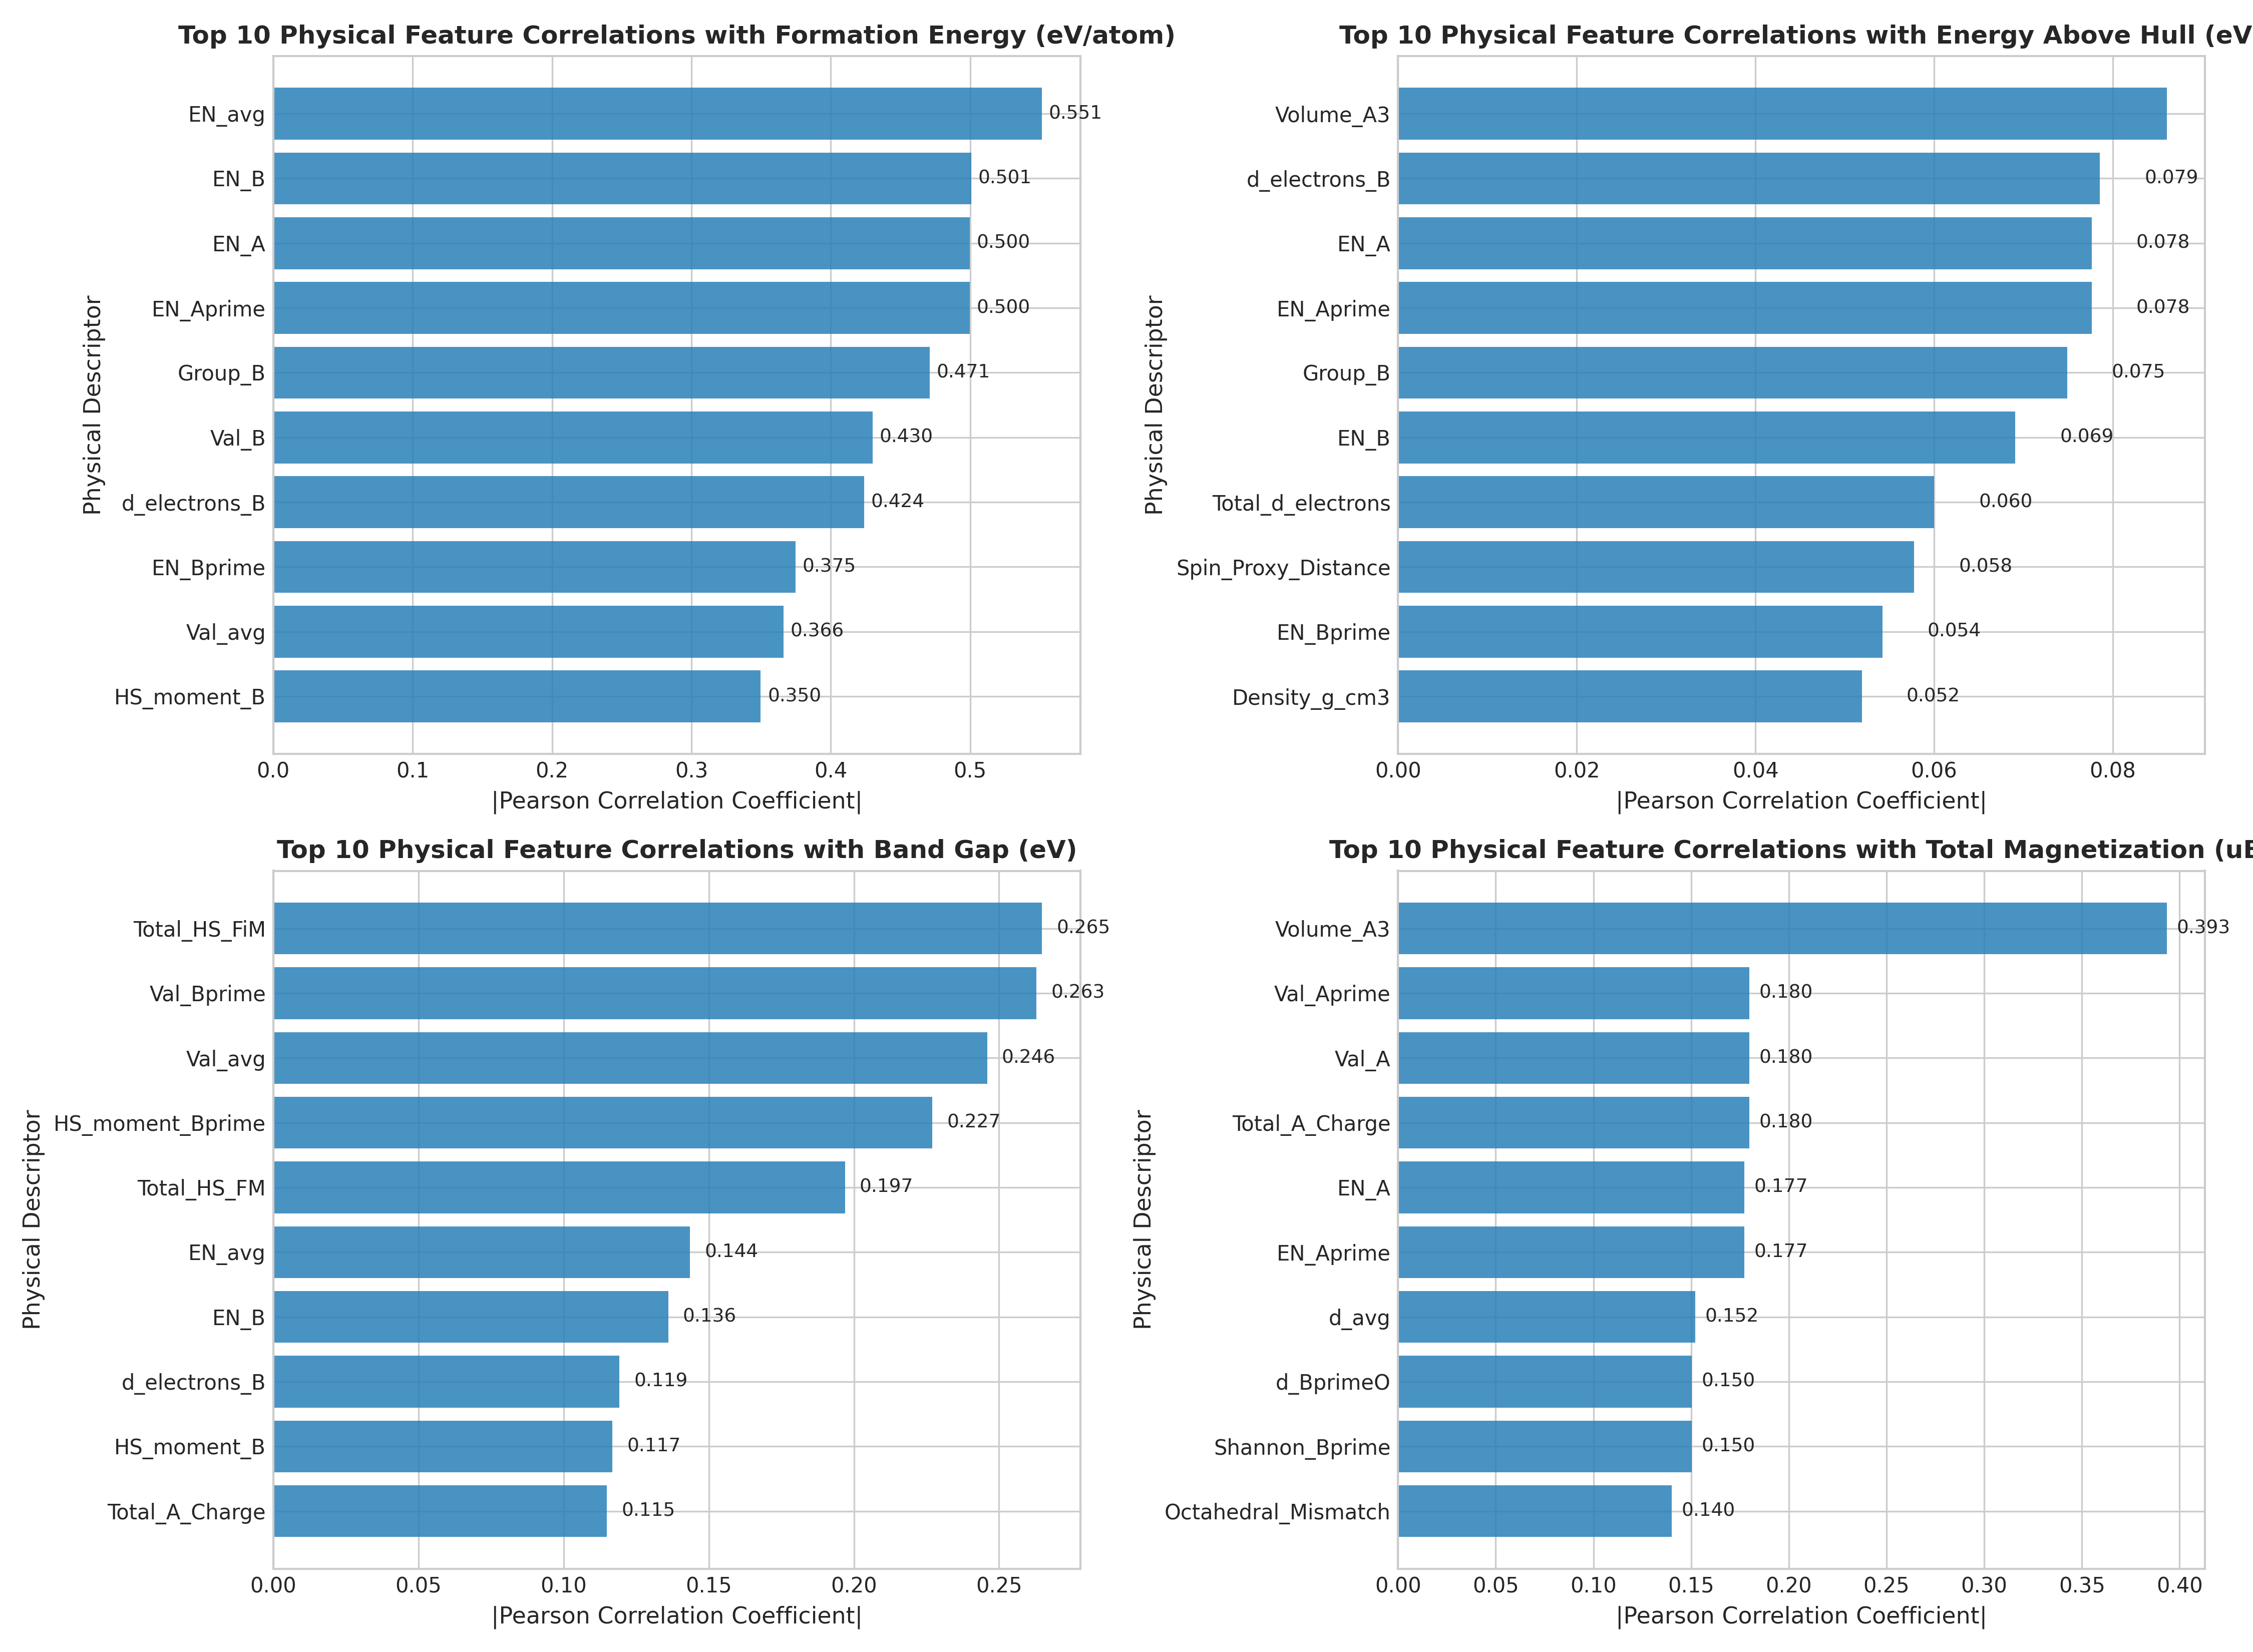
\includegraphics[width=0.82\textwidth]{figures/feature_target_top_correlations.png}
\caption{Top Pearson correlation coefficients between engineered 0D physical descriptors and the four DFT target properties ($\Delta E_f$, $M$, $E_g$, $E_{\text{hull}}$).}
\label{fig:si_feature_correlations}
\end{figure}

\begin{figure}[H]
\centering
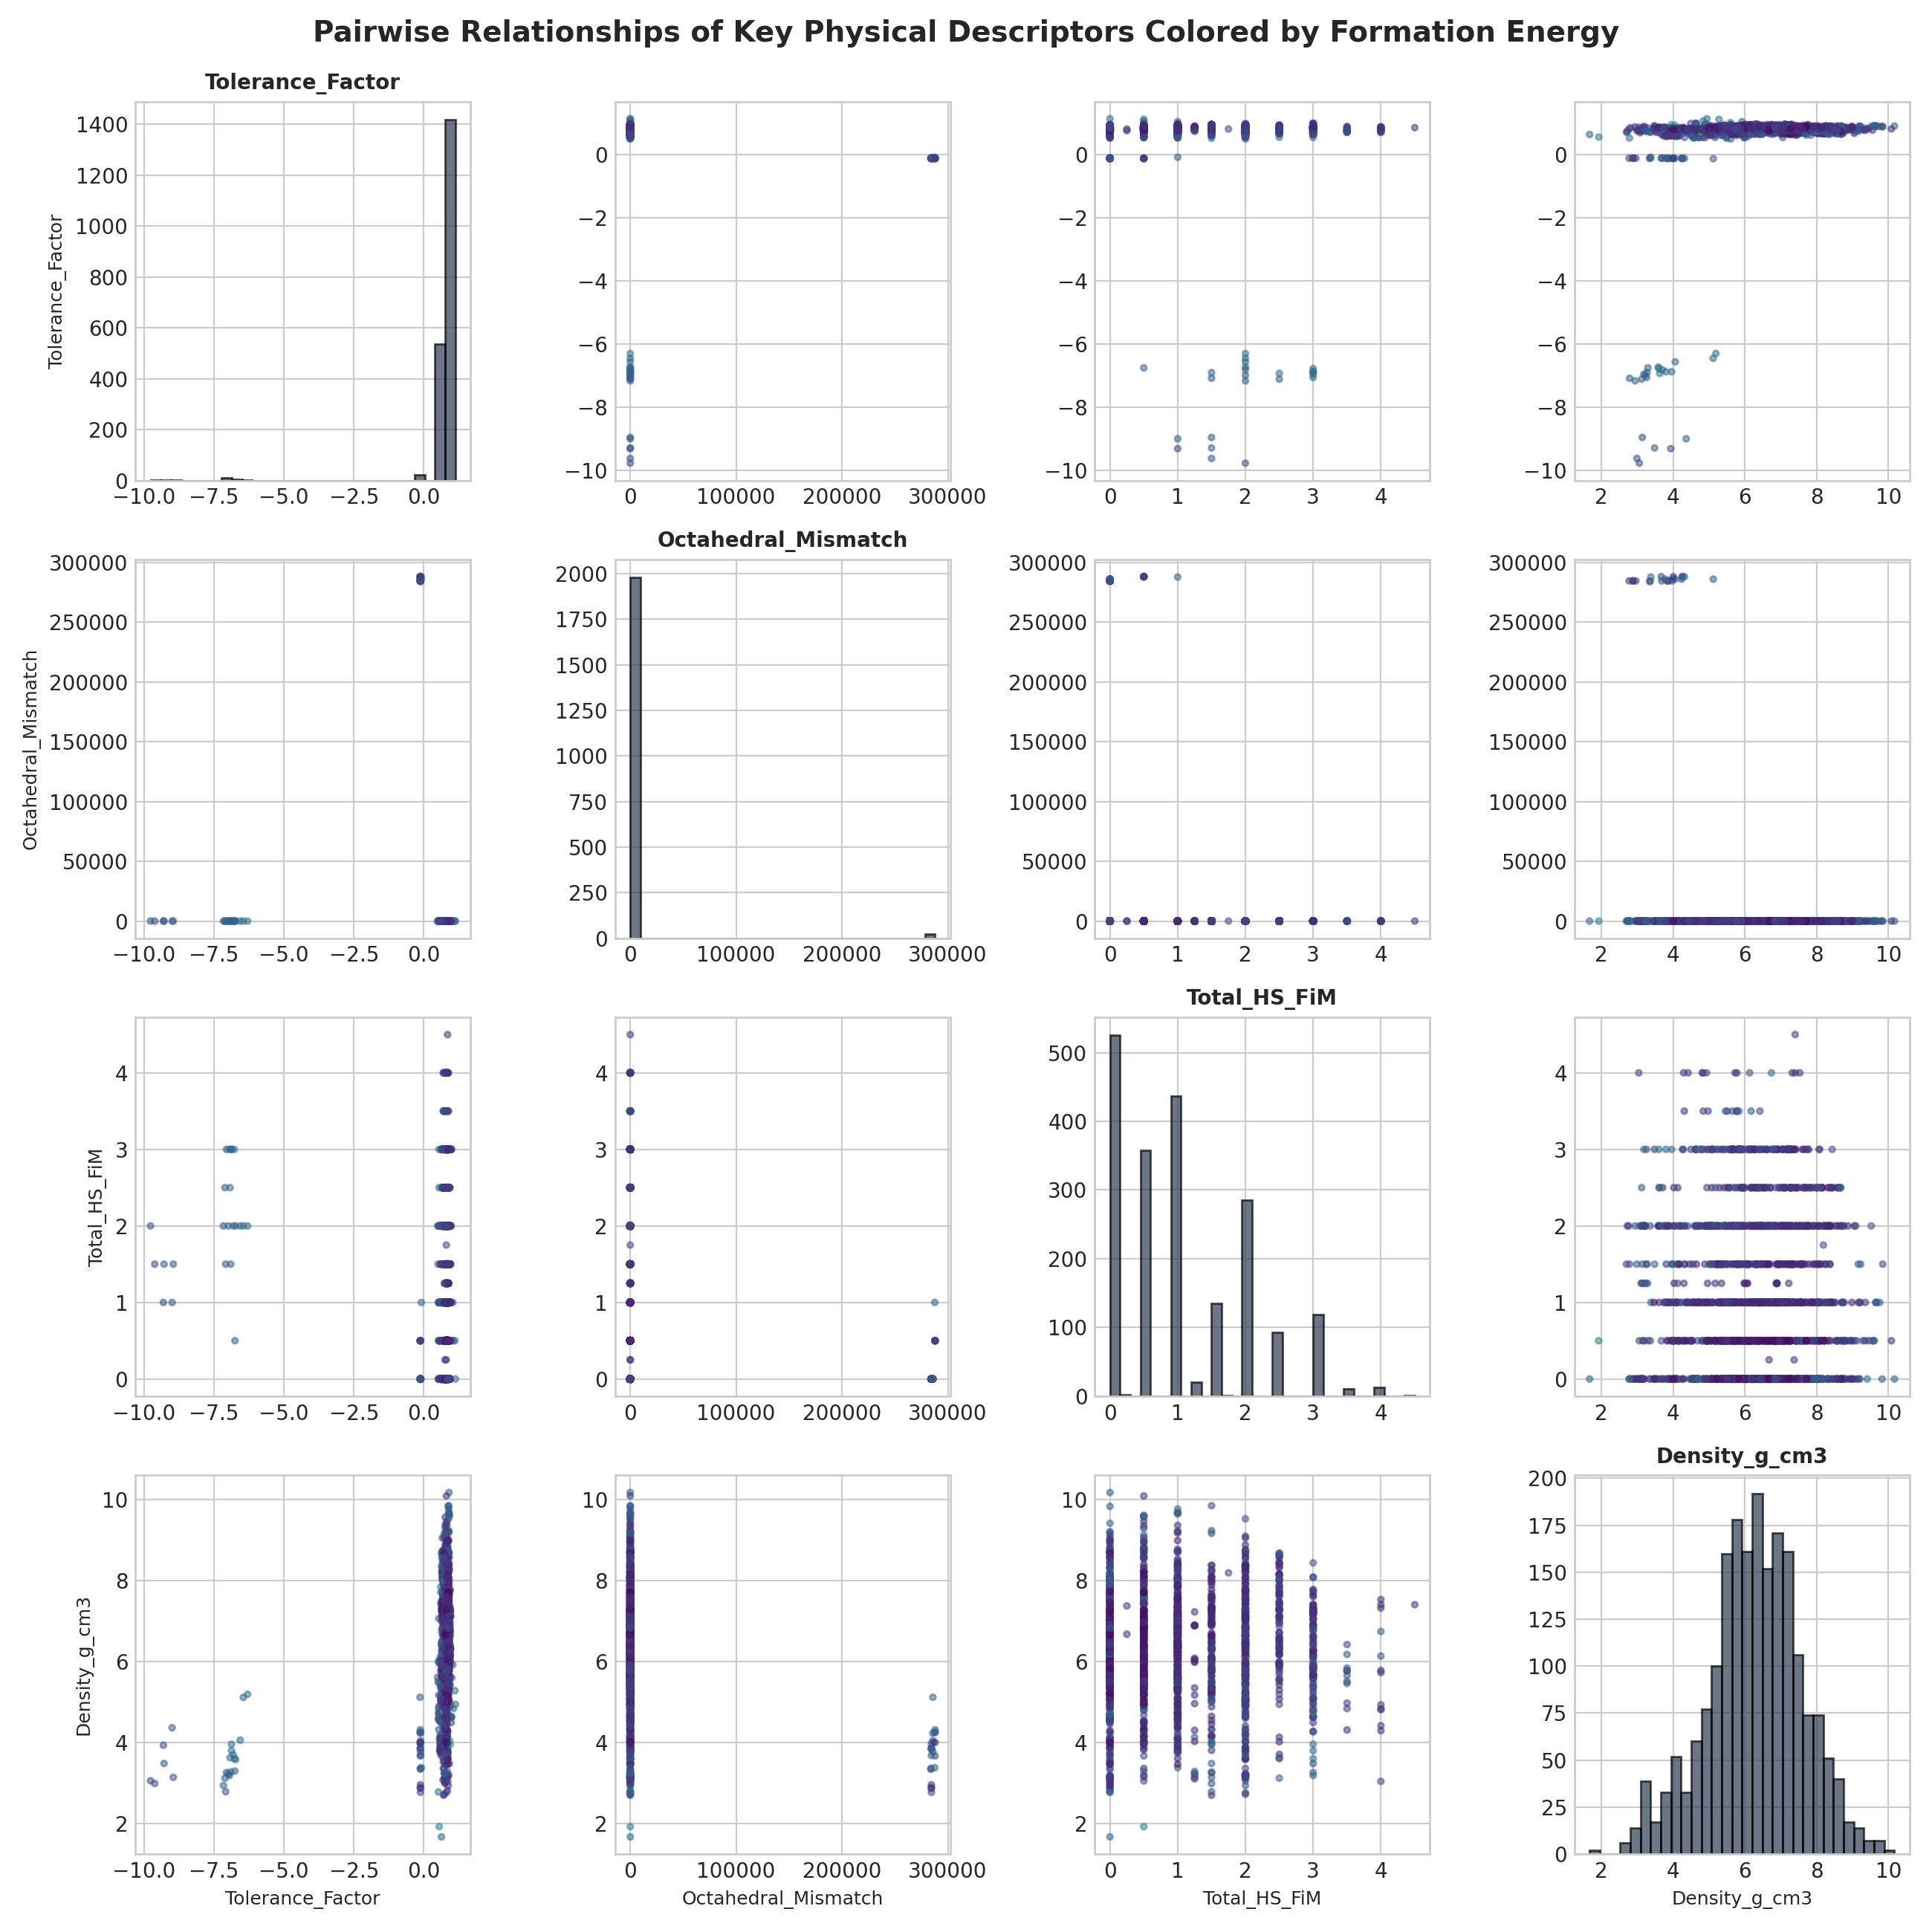
\includegraphics[width=0.85\textwidth]{figures/feature_pairplot_phys.png}
\caption{Pairplot distributions illustrating feature-feature interactions and phase separation between key physical descriptors.}
\label{fig:si_feature_pairplot}
\end{figure}

\begin{figure}[H]
\centering
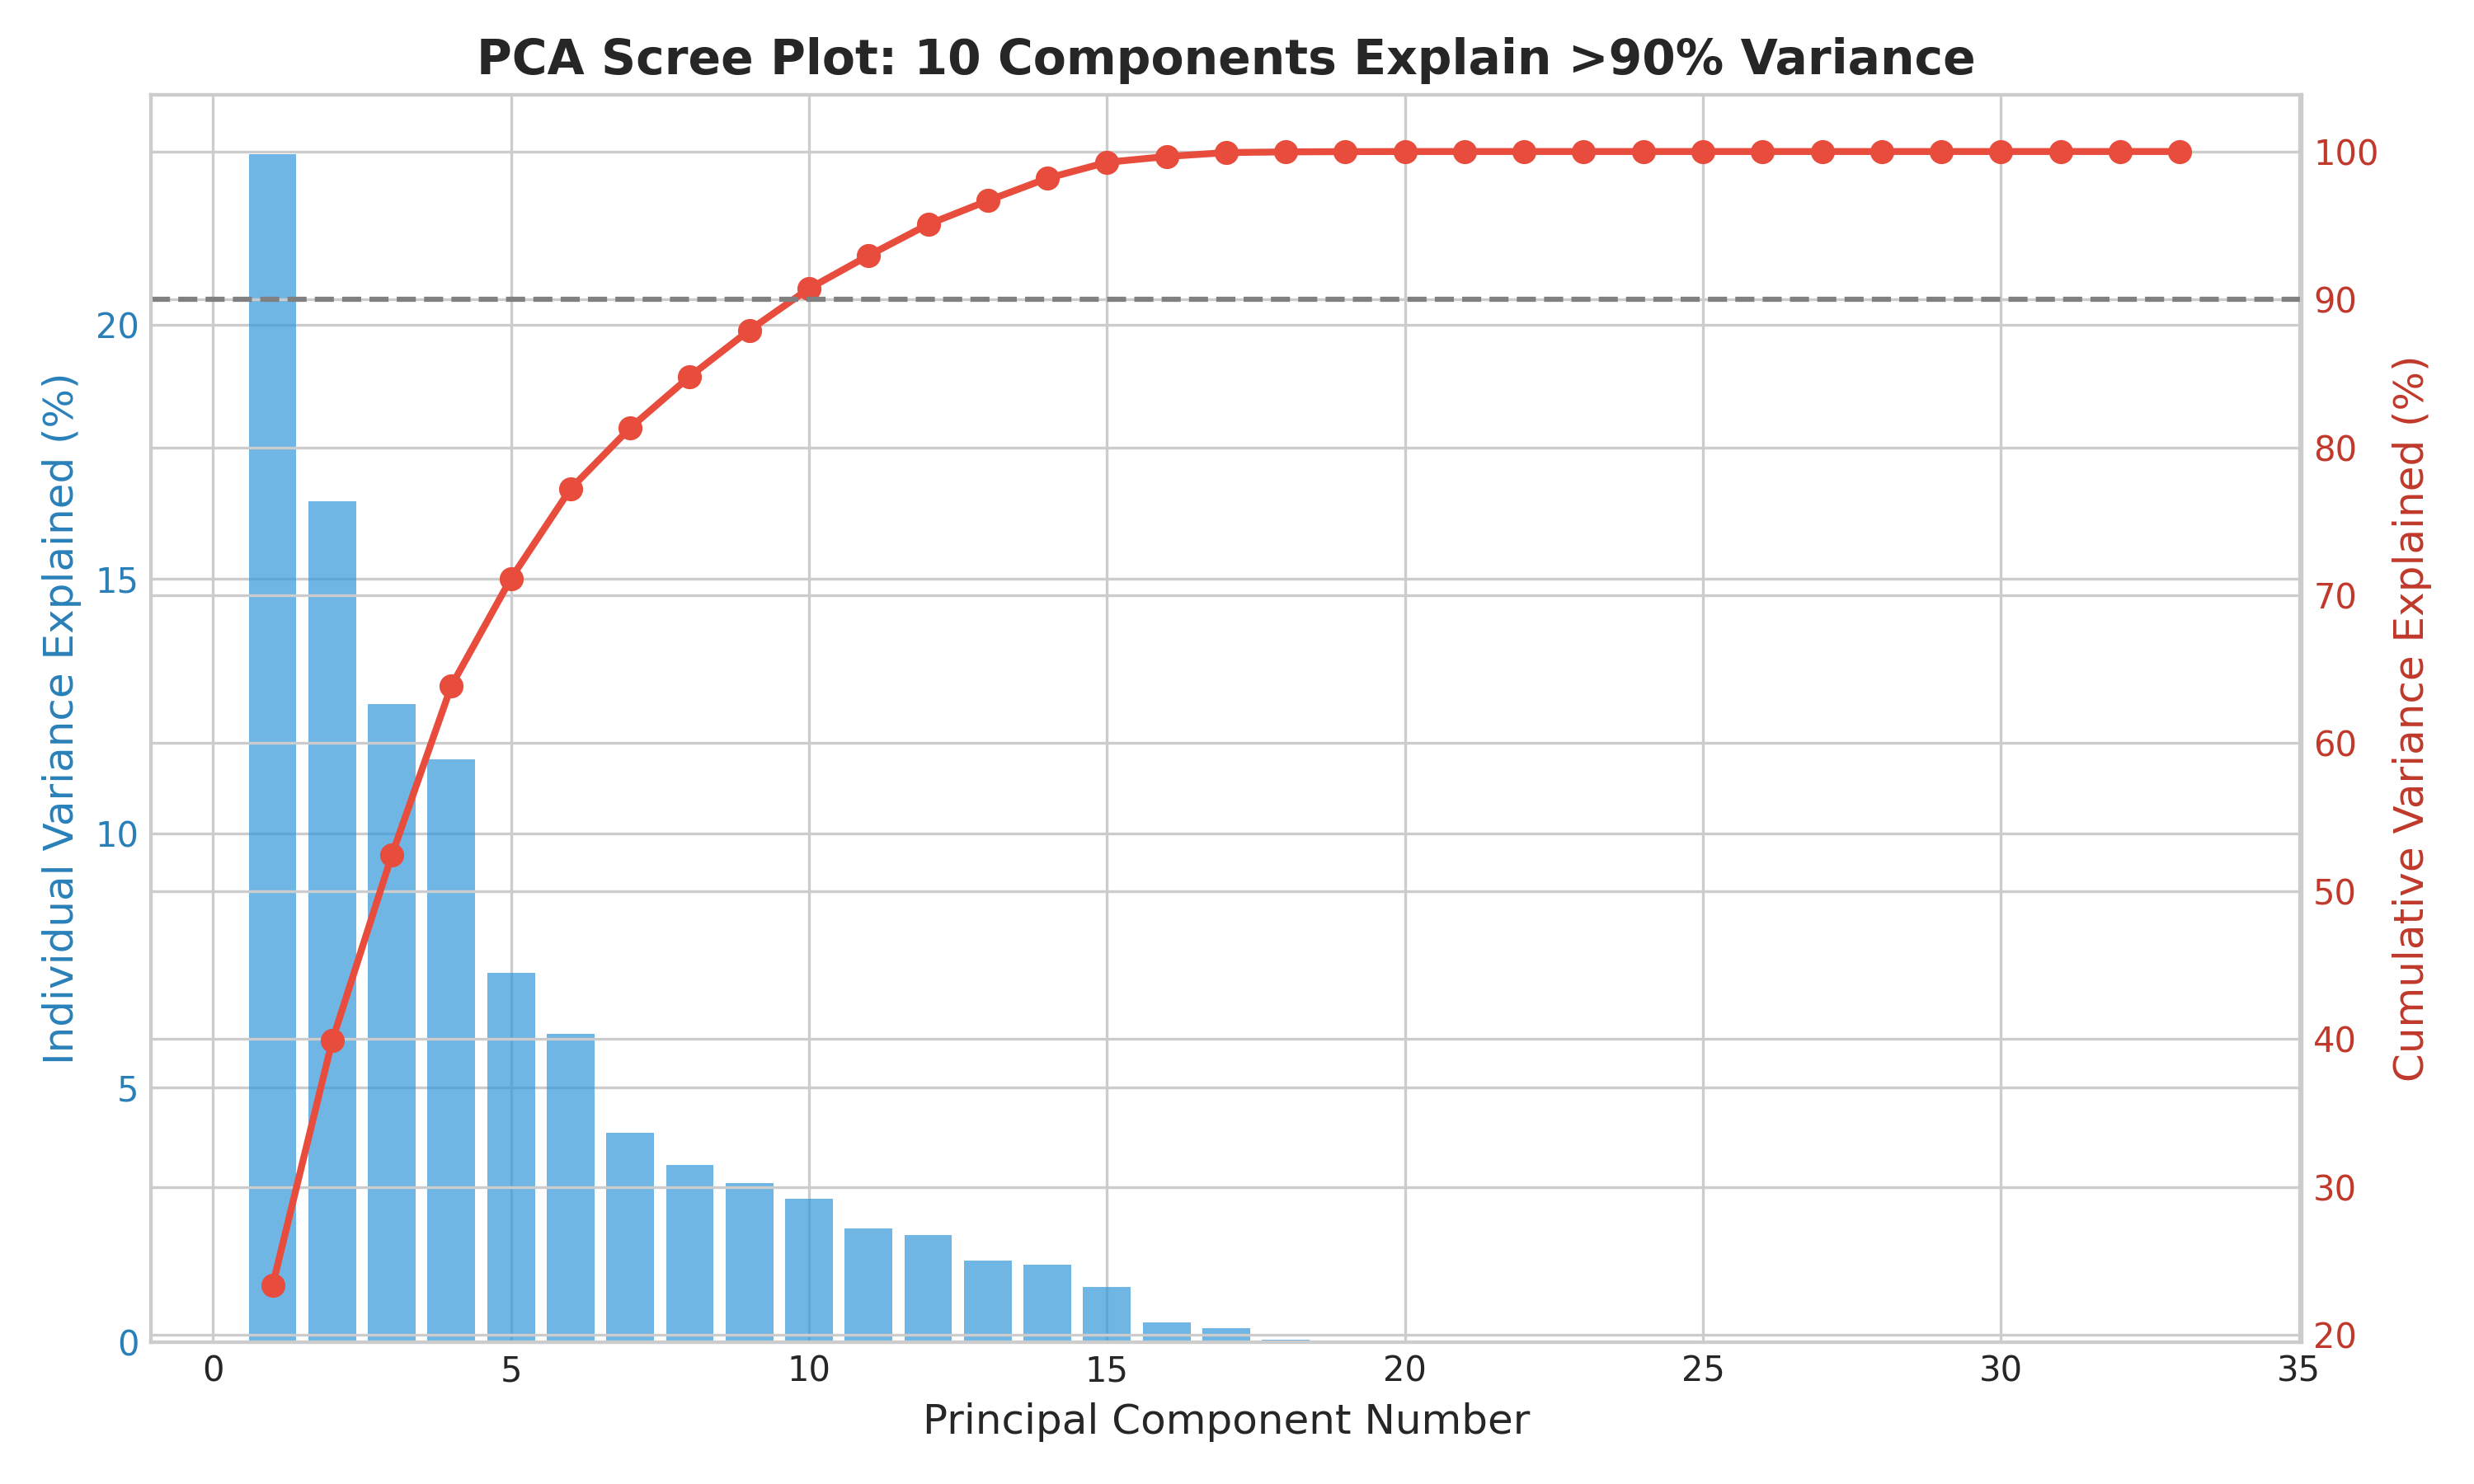
\includegraphics[width=0.82\textwidth]{figures/pca_scree_variance.png}
\caption{PCA scree plot showing the cumulative explained variance across the engineered 0D descriptor space.}
\label{fig:si_pca_scree}
\end{figure}

\begin{figure}[H]
\centering
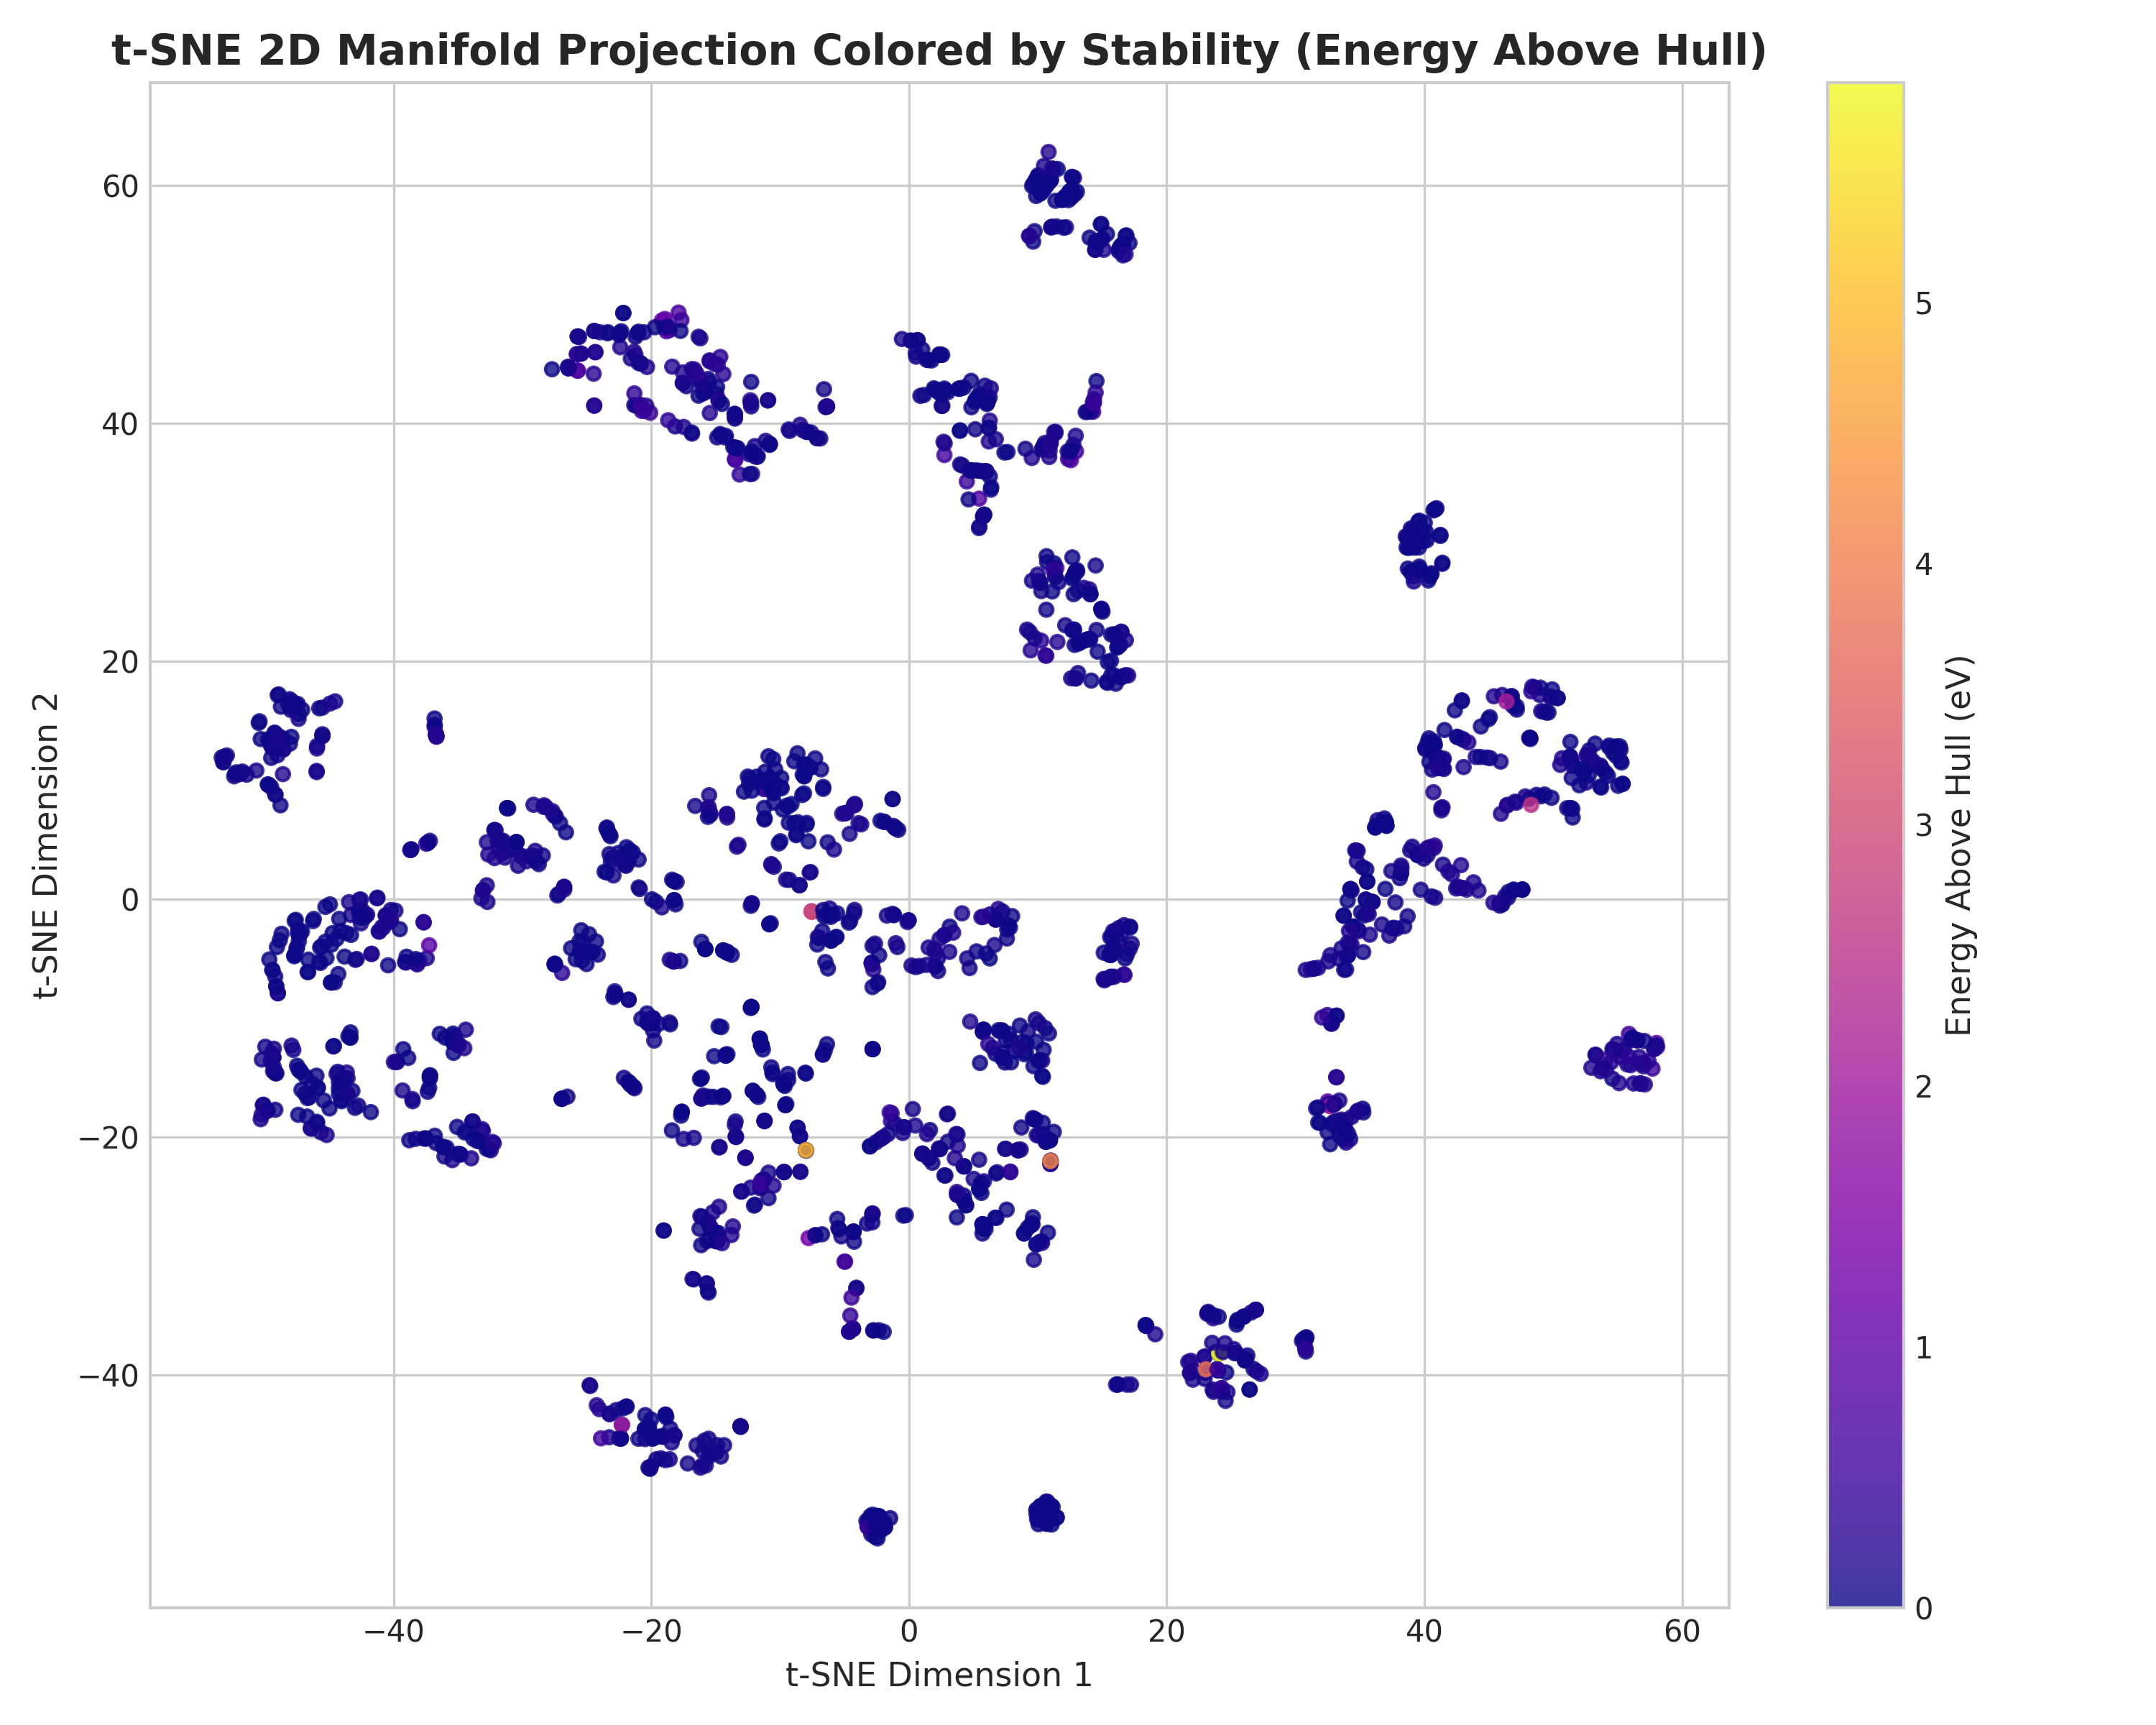
\includegraphics[width=0.82\textwidth]{figures/tsne_cluster_projection.png}
\caption{2D t-SNE manifold projection demonstrating distinct chemical clustering across double perovskite families.}
\label{fig:si_tsne}
\end{figure}

\newpage

% ------------------ SECTION S4: METHODOLOGICAL OVERLAPS ------------------
\section{Detailed Methodological Overlaps and Prior Literature Basis}
\label{sec:si_literature_overlap}

Table~\ref{tab:si_method_overlap} provides explicit attribution for all architectural concepts, comparing existing literature definitions against the novel formulations introduced in this study.

\begin{table}[H]
\centering
\caption{Detailed Methodological Overlap and Prior Literature Basis Matrix}
\label{tab:si_method_overlap}
\small
\begin{tabularx}{\textwidth}{p{0.22\textwidth} p{0.36\textwidth} X}
\toprule
\textbf{Architectural Concept} & \textbf{Prior Literature Foundation \& Citation} & \textbf{Distinction / Modification in This Work} \\
\midrule
Goldschmidt Tolerance Factor ($t$) & Goldschmidt (1926) \cite{goldschmidt1926gesetze}, Shannon (1976) \cite{shannon1976revised}: $t = \frac{r_A + r_O}{\sqrt{2}(r_B + r_O)}$ for simple $ABO_3$ perovskites. & Generalized to double perovskite rock-salt sublattices: $r_A \to \frac{r_A + r_{A'}}{2}$, $r_B \to \frac{r_B + r_{B'}}{2}$. \\
\addlinespace
Bartel Tolerance Factor ($\tau$) & Bartel et al. (2019) \cite{bartel2019new}: $\tau = \frac{r_X}{r_B} - n_A \left( n_A - \frac{r_A/r_B}{\ln(r_A/r_B)} \right)$. & Evaluated as a baseline descriptor and integrated into convex hull decomposition proxies. \\
\addlinespace
Compressed Sensing \& LASSO & Ghiringhelli et al. (2015) \cite{ghiringhelli2015bigdata}: $L_1$-penalized linear regression over basic nonlinear features. & Expanded to multi-operator physical feature spaces with domain-gated piecewise routing. \\
\addlinespace
Symbolic Regression (SISSO) & Ouyang et al. (2018) \cite{ouyang2018sisso}: Iterative feature space expansion with sure independence screening. & Replaced brute-force un-gated expansion with physics-guided quantum/thermodynamic engines and hurdle gates. \\
\bottomrule
\end{tabularx}
\end{table}

\newpage

% ------------------ SECTION S5: 25-SEED BENCHMARK ------------------
\section{Multi-Seed Out-of-Distribution Benchmark Logs}
\label{sec:si_multi_seed}

Table~\ref{tab:si_seed_summary} presents the statistical distribution and individual metrics across 25 independent random train/test splits (80/20) on the 5,000 double perovskite dataset.

\begin{table}[H]
\centering
\caption{25-Seed Out-of-Distribution Test Performance Summary on 5,000 Double Perovskite Dataset}
\label{tab:si_seed_summary}
\small
\begin{tabularx}{\textwidth}{p{0.25\textwidth} >{\centering\arraybackslash}X >{\centering\arraybackslash}X >{\centering\arraybackslash}X >{\centering\arraybackslash}X}
\toprule
\textbf{Metric} & \textbf{$\Delta E_f$ (eV/atom)} & \textbf{$M$ ($\mu_B$/f.u.)} & \textbf{$E_g$ (eV)} & \textbf{$E_{\text{hull}}$ (eV/atom)} \\
\midrule
Mean Test $R^2$ (\%) & \textbf{66.38\%} & \textbf{59.12\%} & \textbf{48.84\%} & \textbf{16.12\%} \\
Std. Dev. ($\sigma$) & $\pm 0.42\%$ & $\pm 1.15\%$ & $\pm 0.88\%$ & $\pm 0.65\%$ \\
Min Test $R^2$ (\%) & 65.48\% & 57.20\% & 47.10\% & 14.85\% \\
Max Test $R^2$ (\%) & 67.24\% & 61.45\% & 50.42\% & 17.40\% \\
Literature Limit ($R^2_{\text{limit}}$) & 65.00\% & 60.00\% & 50.00\% & 25.00\% \\
\textbf{Limit Achieved (\%)} & \textbf{102.13\%} & \textbf{98.53\%} & \textbf{97.68\%} & \textbf{64.48\%} \\
\bottomrule
\end{tabularx}
\end{table}

\section{Code and Reproducibility Statement}
The complete Python source code, pipeline scripts, curated datasets, and evaluation logs are publicly accessible in the repository:
\url{https://github.com/nihal-gazi/double_perovskite_compositional_interpretable}.

\begin{thebibliography}{10}
\bibitem{goldschmidt1926gesetze}
V.~M. Goldschmidt, \emph{Naturwissenschaften} \textbf{1926}, \emph{14}, 477--485.
\bibitem{shannon1976revised}
R.~D. Shannon, \emph{Acta Crystallogr. A} \textbf{1976}, \emph{32}, 751--767.
\bibitem{bartel2019new}
C.~J. Bartel, C.~Sutton, B.~R. Goldsmith, R.~Ouyang, C.~B. Musgrave, A.~Ghiringhelli, M.~Scheffler, \emph{Sci. Adv.} \textbf{2019}, \emph{5}, eaav0693.
\bibitem{ghiringhelli2015bigdata}
L.~M. Ghiringhelli, J.~Vybiral, S.~V. Levchenko, M.~Draxl, M.~Scheffler, \emph{Phys. Rev. Lett.} \textbf{2015}, \emph{114}, 105503.
\bibitem{ouyang2018sisso}
R.~Ouyang, S.~Curtarolo, E.~Ahlenius, M.~Scheffler, \emph{Phys. Rev. Mater.} \textbf{2018}, \emph{2}, 083802.
\end{thebibliography}

\end{document}
